\documentclass[lettersize,journal]{IEEEtran}
\usepackage{amsmath,amsfonts}
\usepackage{algorithmic}
\usepackage{algorithm}
\usepackage{array}
\usepackage[caption=false,font=normalsize,labelfont=sf,textfont=sf]{subfig}
\usepackage{textcomp}
\usepackage{stfloats}
\usepackage{url}
\usepackage{verbatim}
\usepackage{graphicx}
\usepackage{cite}
\usepackage{tikz}
\usetikzlibrary{positioning, calc, shapes, arrows, fit}
\usepackage{circuitikz}
\hyphenation{op-tical net-works semi-conduc-tor IEEE-Xplore}
\graphicspath{{images/}}
% updated with editorial comments 8/9/2021

\begin{document}

\title{Lab 2 -- Generating and Measuring Waveforms}

\author{Benjamin Sage\\Lab Partners: Marc Huerta, Devorah Simon}

% The paper headers
\markboth{EE 133: Analog Communications Design Laboratory, February~2022}%
{Shell \MakeLowercase{\textit{et al.}}: A Sample Article Using IEEEtran.cls for IEEE Journals}

% \IEEEpubid{0000--0000/00\$00.00~\copyright~2021 IEEE}
% Remember, if you use this you must call \IEEEpubidadjcol in the second
% column for its text to clear the IEEEpubid mark.

\maketitle

\begin{abstract}
A microprocessor was used to generate three distinct types of waveforms at three separate frequencies. The waveforms were then analyzed using an oscilloscope. Finally, a spectrum analyzer ran a fourier transform on the wave to verify the frequency.
\end{abstract}

% \begin{IEEEkeywords}
% Article submission, IEEE, IEEEtran, journal, \LaTeX, paper, template, typesetting.
% \end{IEEEkeywords}

\section{Introduction}
\IEEEPARstart{M}{odern} wave form generation often has two components:

\begin{itemize}
    \item A clock generator
    \item A microcontroller
\end{itemize}

This setup has the advantage of being low-cost and also generally reliable.

In this lab, we will use an Si5351 clock generator and ItsyBitsy microcontroller to generate waveforms which can be analyzed on an oscillocsope. With just this setup, we will be able to generate several different frequencies of waveform.

The microcontroller will be programmed in a Python-like language called CircuitPython, which is open-source an easy to pick up for beginners.


\section{Experimental Setup}

The setup for this lab is a bit technical on both the signal generator and microprocessor sides. So I will enumerate the steps.

\begin{enumerate}
    \item Gathered materials: Adafruit ItsyBitsy M4 Express, Adafruit Si5351A Clock Generator, breadboard, jumper cables.
    \item Soldered SMA connectors to both the ItsyBitsy and the Si5351A.
    \item Attached both ItsyBitsy and Si5351A to breadboard.
    \item Connected appropriate pins between ItsyBitsy and Si5351A using jumper cables. (Correct pins can be seen in Fig. 1. and {\bf{Table 1}}.)
    \item Downloaded the Mu Editor for programming the ItsyBitsy microcontroller.
    \item Updated the bootloader on the ItsyBitsy.
    \item Installed CircuitPython to the ItsyBitsy.
\end{enumerate}

\begin{table}
\renewcommand{\arraystretch}{2.2}
\begin{center}
\caption{ItsyBitsy and Si5351A Port Connections}
\label{tab1}
\begin{tabular}{c c}
\hline
\bfseries ItsyBitsy Pin & \bfseries Si5351A Pin\\
\hline
3V & Vin\\
\hline
GND & GND\\ 
\hline
SCL & SCL\\
\hline 
SDA& SDA\\
\hline
\end{tabular}
\end{center}
\end{table}

\begin{figure}[!t]
\centering
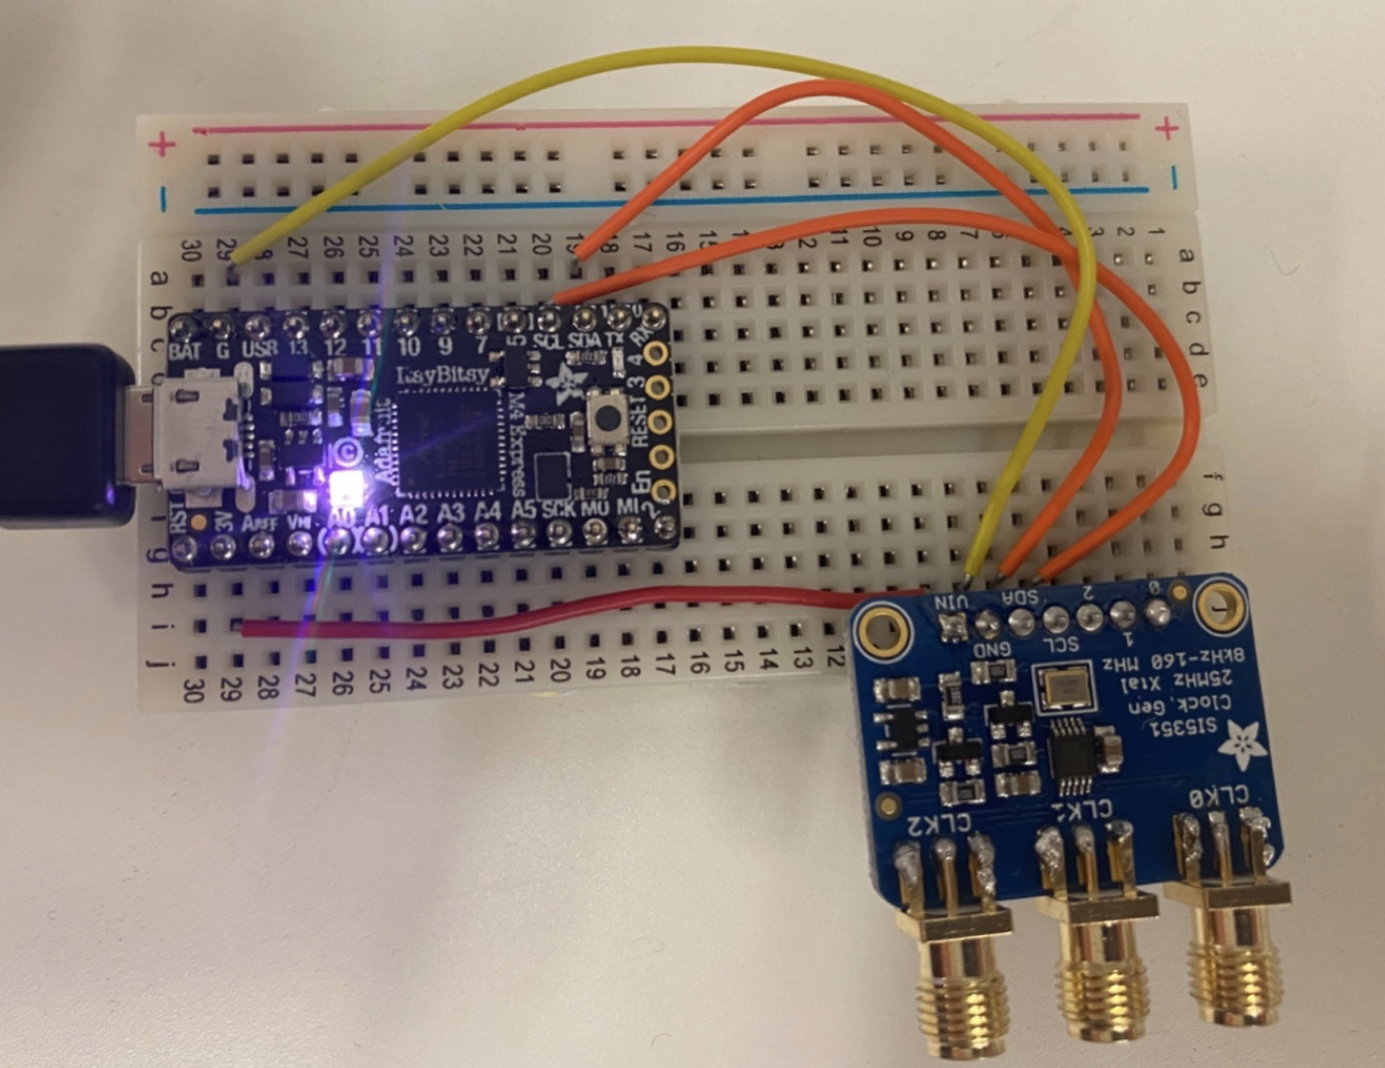
\includegraphics[width=2.5in]{cables}
\caption{ItsyBitsy, Si5351A, and breadboard connected using appropriate ports, as described in the documentation.}
\label{fig_1}
\end{figure}

\section{Measurements and Results}

Using the setup, we generated three different waveforms:

\begin{itemize}
    \item $112.5\,\text{MHz}$, seen in Fig. 2(a).
    \item $13.55\,\text{MHz}$, seen in Fig. 2(b).
    \item $10.76\,\text{kHz}$, seen in Fig. 2(c).
\end{itemize}

Each waveform was visualized using the oscilloscope. We then compared the measured frequencies from the nominal frequencies, and computed the error. The results are in {\bf{Table 2}}.

\begin{table}
\renewcommand{\arraystretch}{2.2}
\begin{center}
\caption{Oscilliscope Waveform Frequencies}
\label{tab1}
\begin{tabular}{c c c}
\hline
\bfseries Nominal (Hz) & \bfseries Actual (Hz) & \bfseries Error\\
\hline
$1.125 \times 10^{8}$ & $1.119 \times 10^{8} $ & 0.5\%\\
\hline
$1.355 \times 10^{7}$ & $1.351 \times 10^{7}$ & 0.3\%\\ 
\hline
$1.076 \times 10^{4}$ & $1.069 \times 10^{4}$ & 0.7\%\\
\hline
\end{tabular}
\end{center}
\end{table}

\begin{table}
\renewcommand{\arraystretch}{2.2}
\begin{center}
\caption{Spectrum Analyzer Frequency Peaks}
\label{tab1}
\begin{tabular}{c c c}
\hline
\bfseries Nominal (Hz) & \bfseries Actual (Hz) & \bfseries Error\\
\hline
$1.125 \times 10^{8}$ & $1.120 \times 10^{8} $ & 0.4\%\\
\hline
$1.355 \times 10^{7}$ & $1.356 \times 10^{7}$ & 0.1\%\\ 
\hline
$1.076 \times 10^{4}$ & $1.069 \times 10^{4}$ & 0.7\%\\
\hline
\end{tabular}
\end{center}
\end{table}

\begin{figure*}[!t]
\centering
\subfloat[]{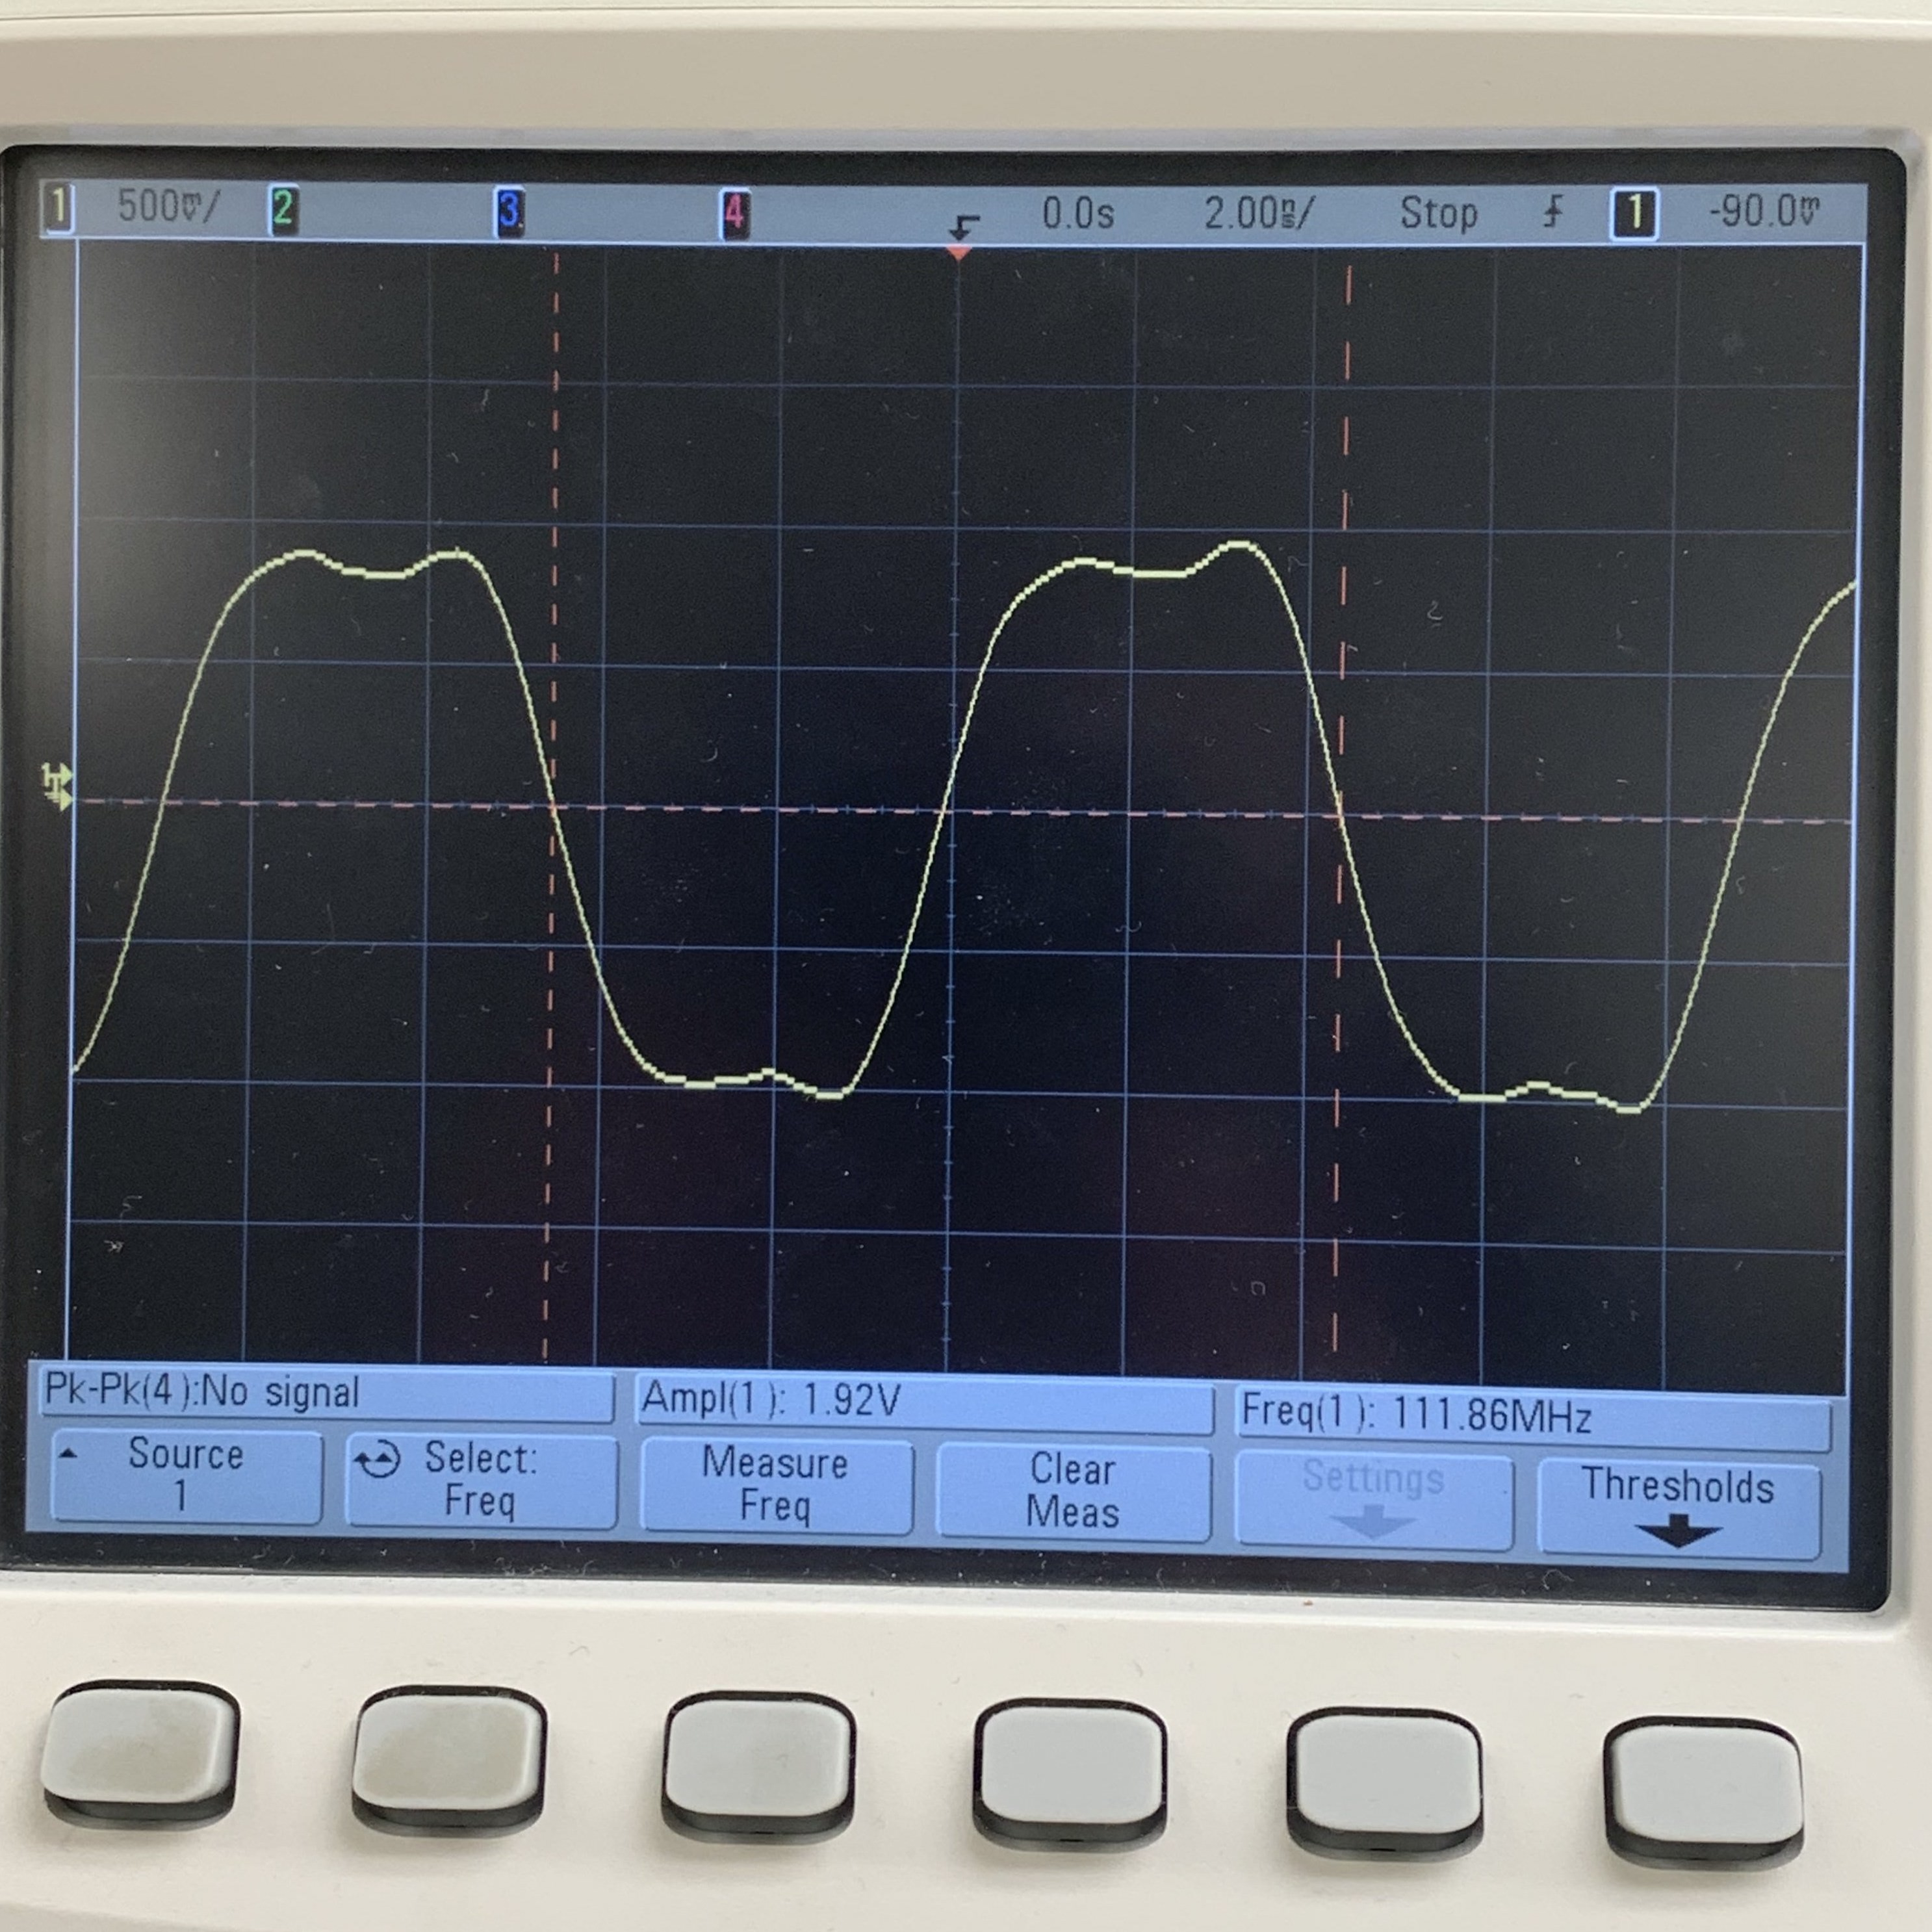
\includegraphics[width=2in]{113}%
\label{fig_first_case}}
\hfil
\subfloat[]{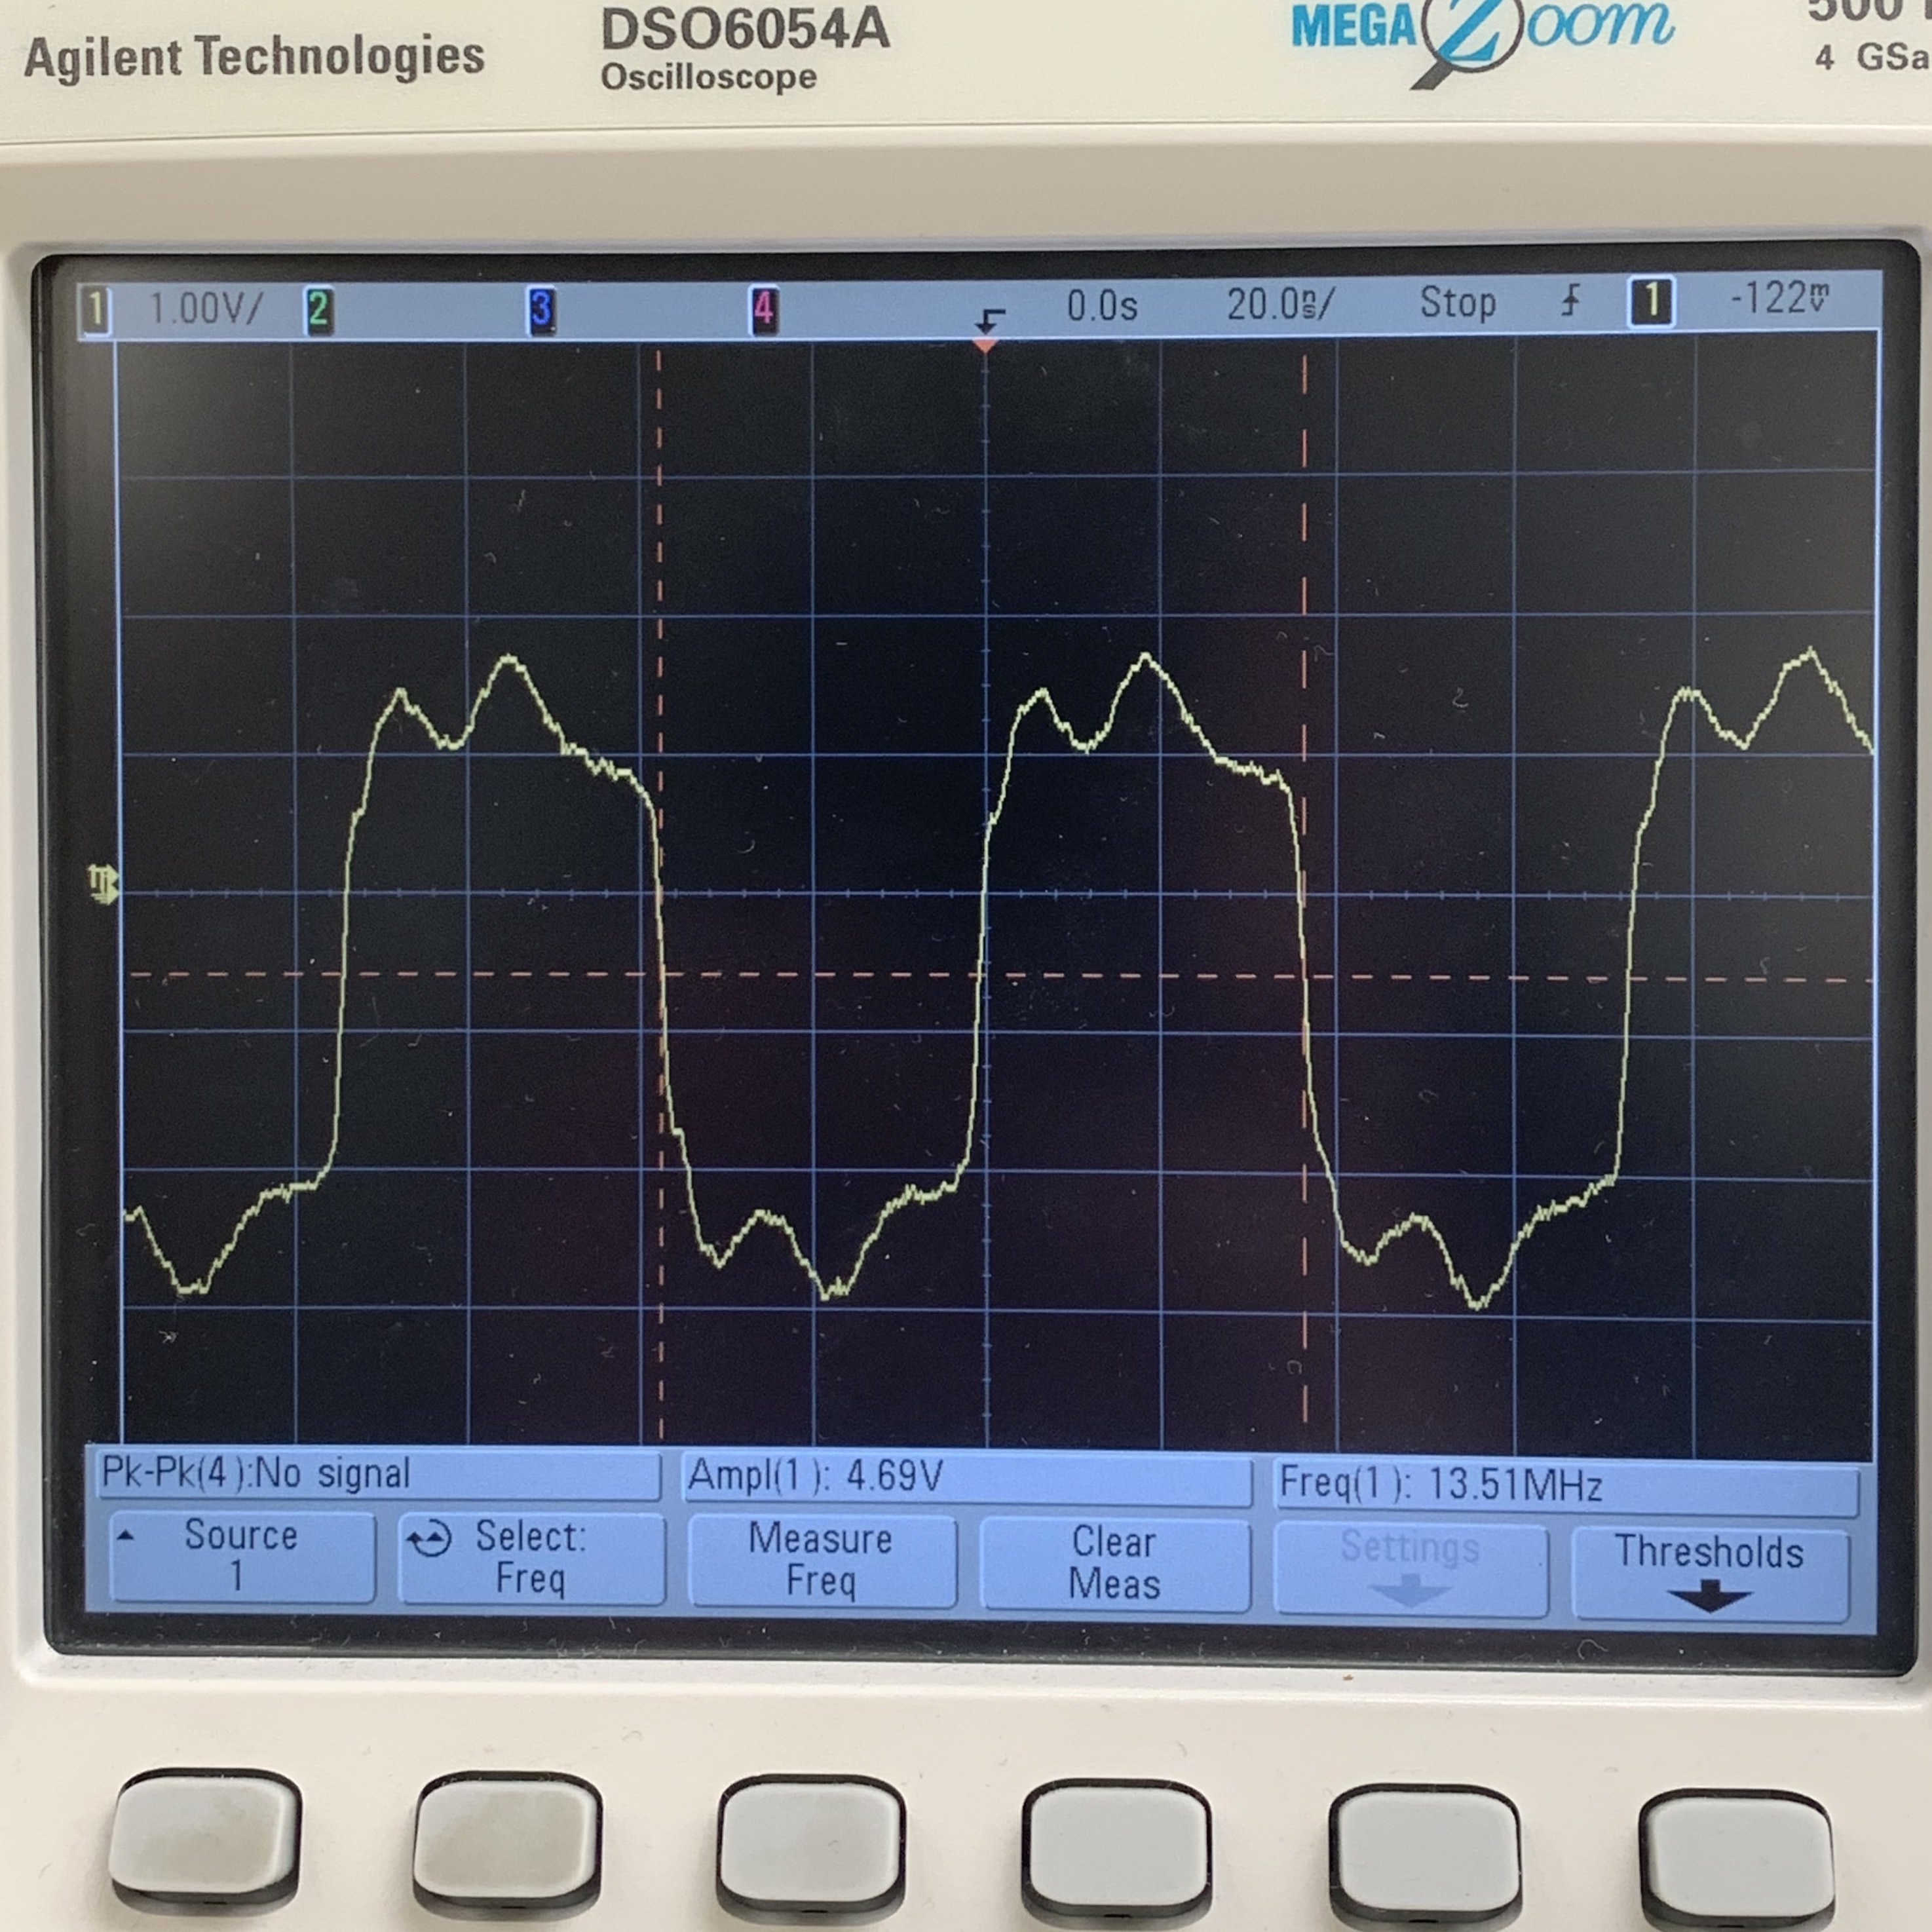
\includegraphics[width=2in]{14}%
\label{fig_second_case}}
\hfil
\subfloat[]{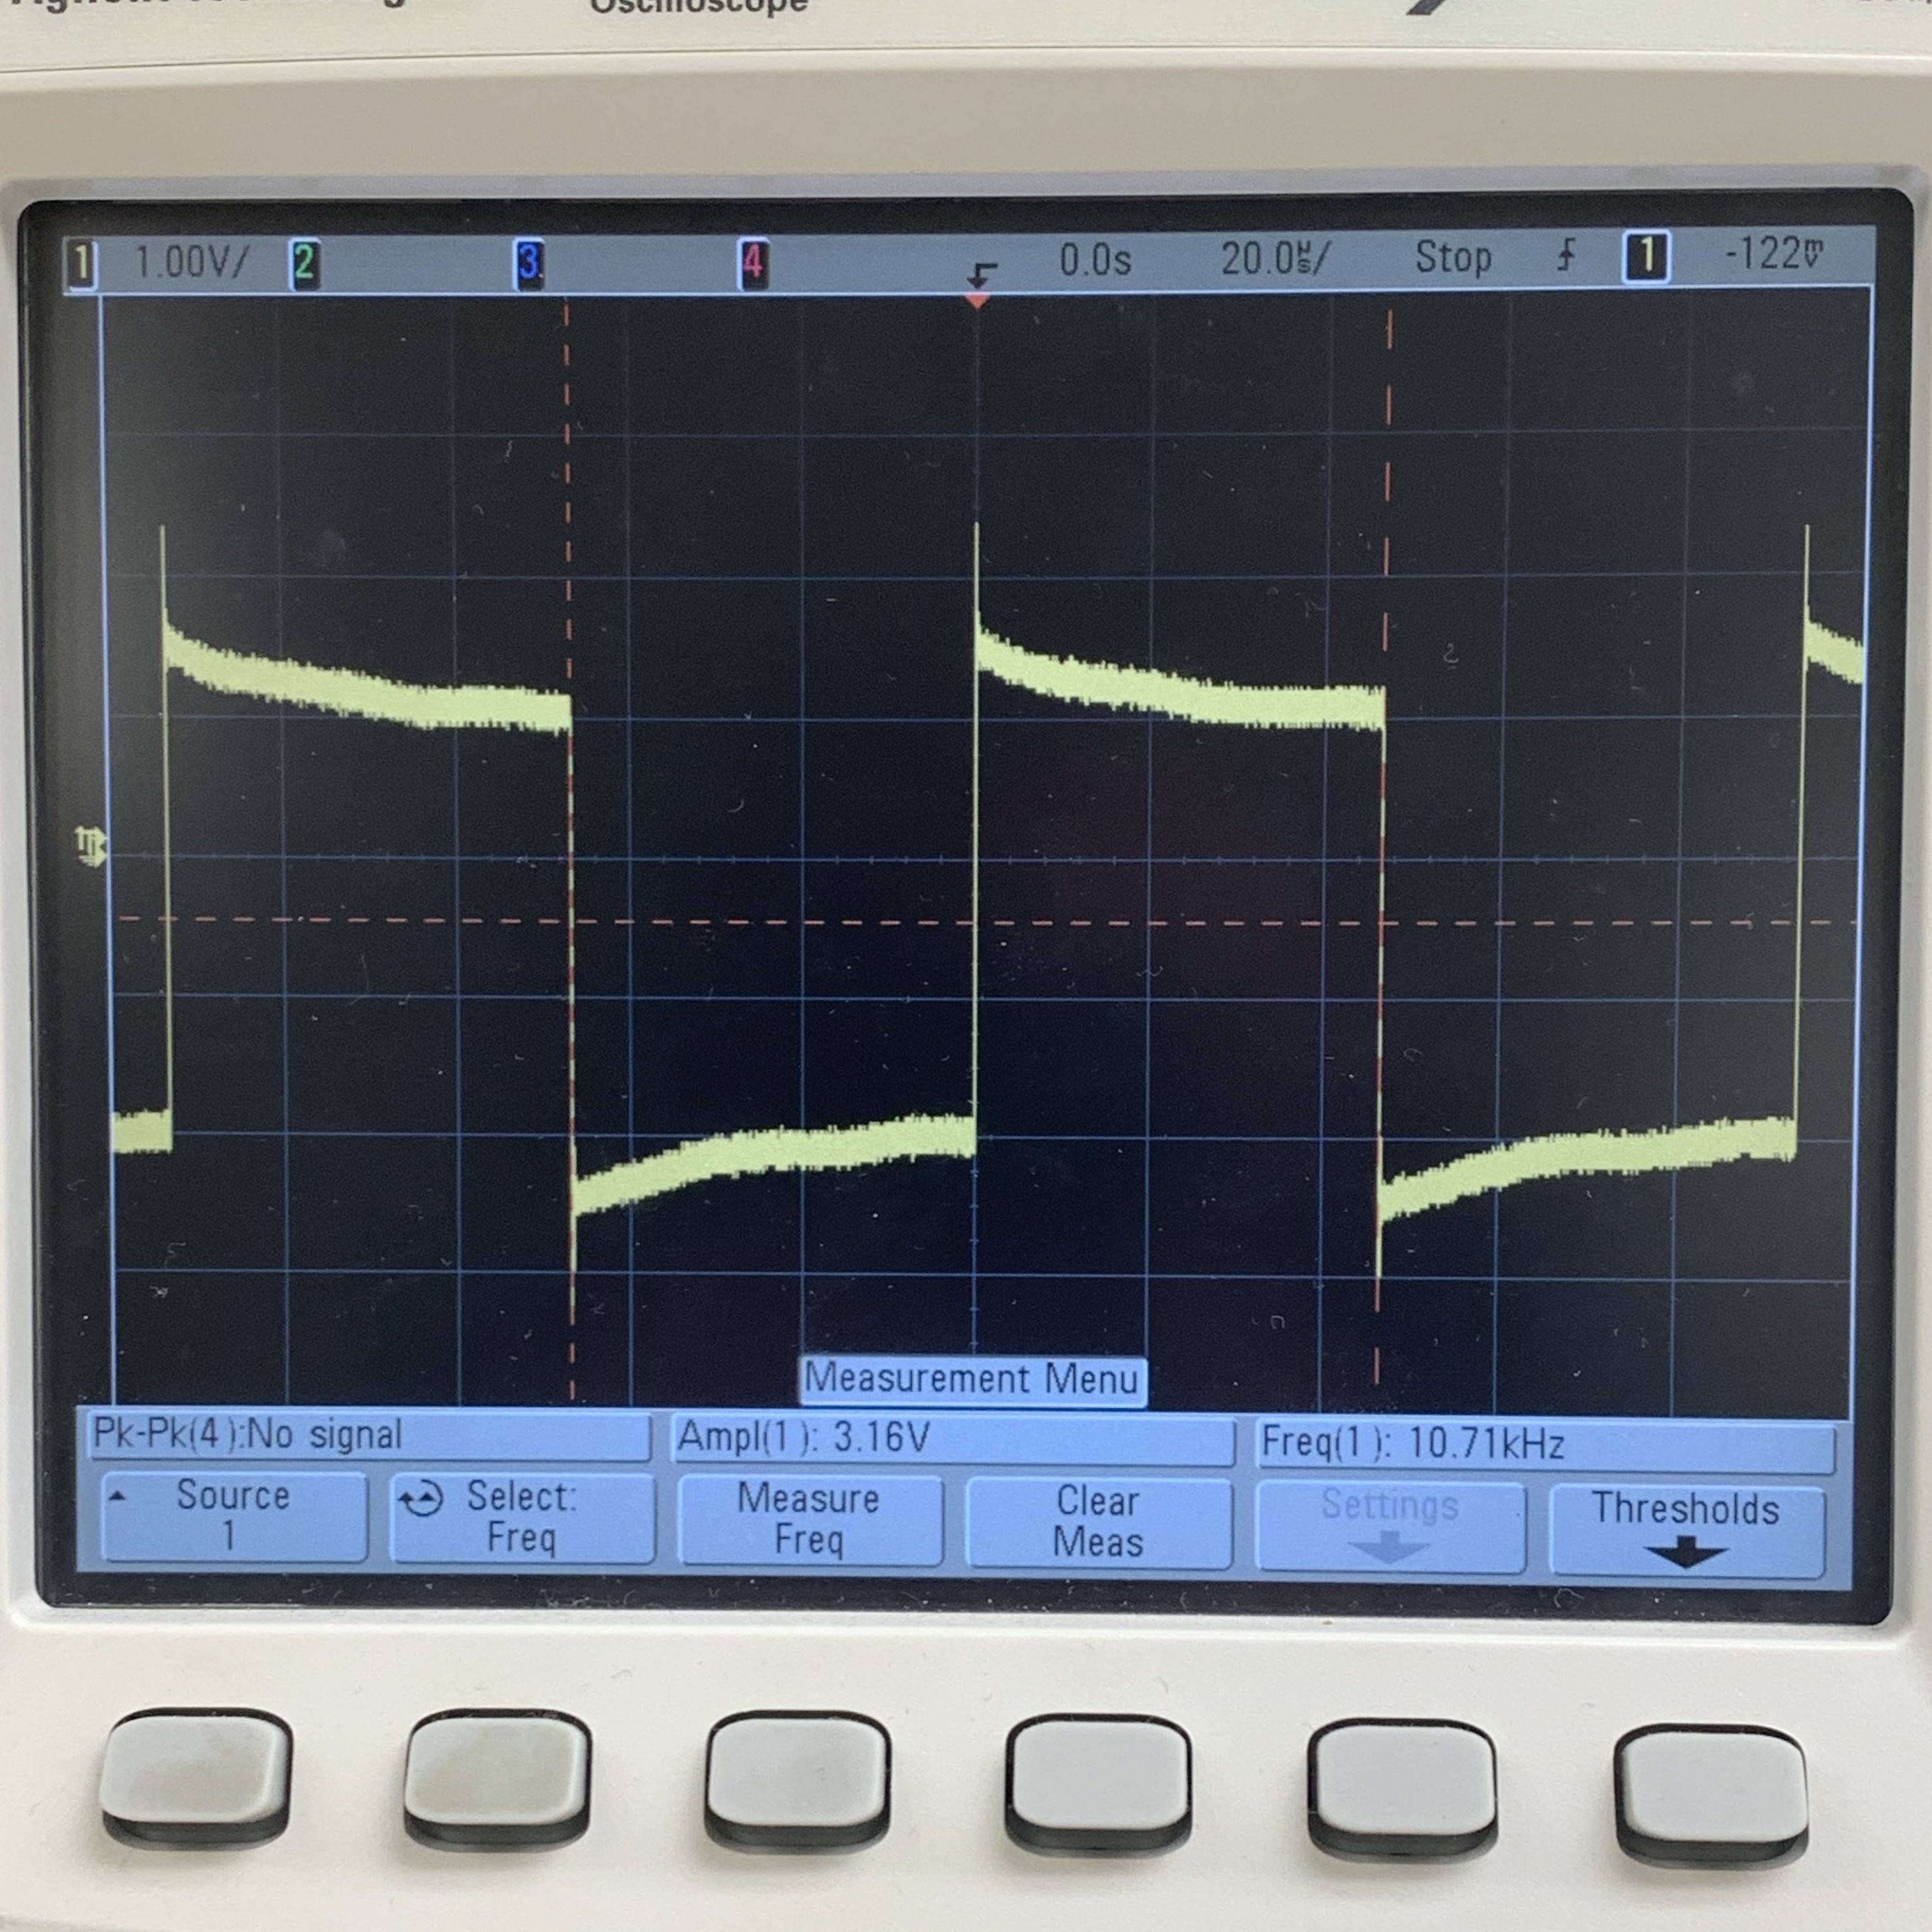
\includegraphics[width=2in]{11}%
\label{fig_third_case}}
\caption{Waveform outputs, as seen with the oscilloscope. (a) $112.5 \,\text{MHz}$. (b) $13.55 \, \text{MHz}$. (c) $10.76 \, \text{kHz}$. Deviations from nominal frequencies can be seen in {\bf{Table 2}}.}
\label{fig_sim}
\end{figure*}

\begin{figure*}[!t]
\centering
\subfloat[]{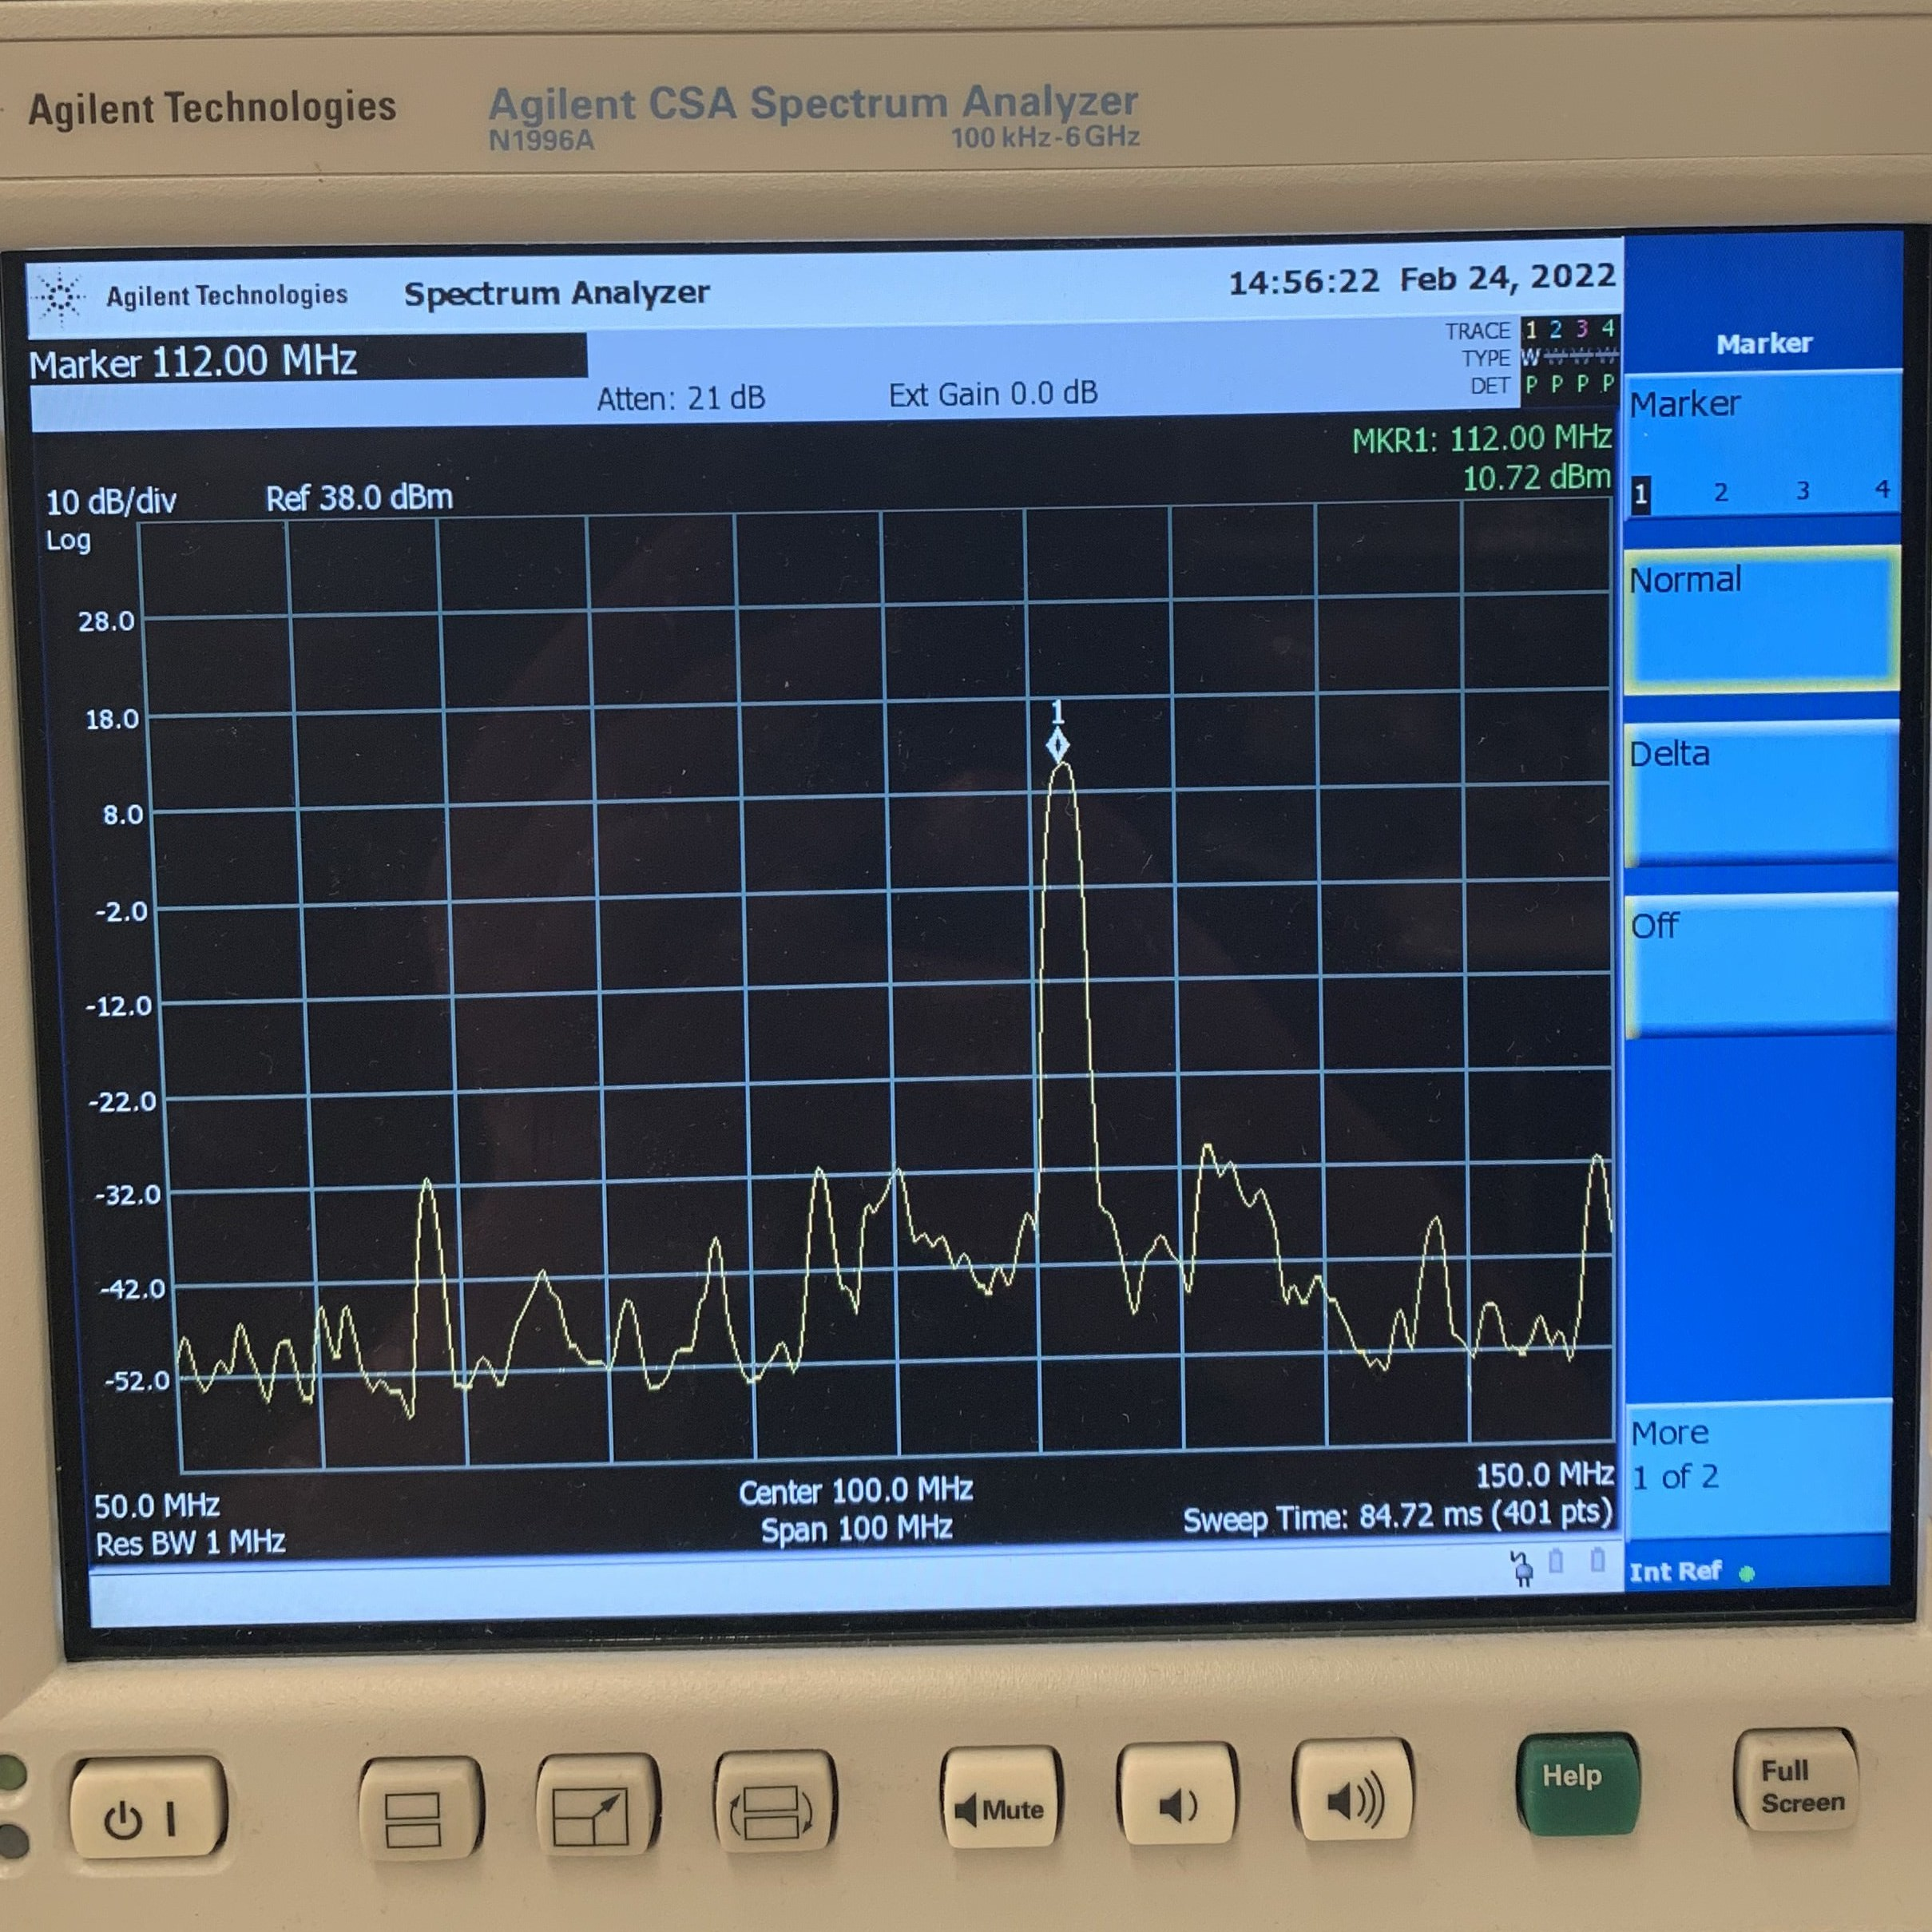
\includegraphics[width=2in]{113f}%
\label{fig_first_case}}
\hfil
\subfloat[]{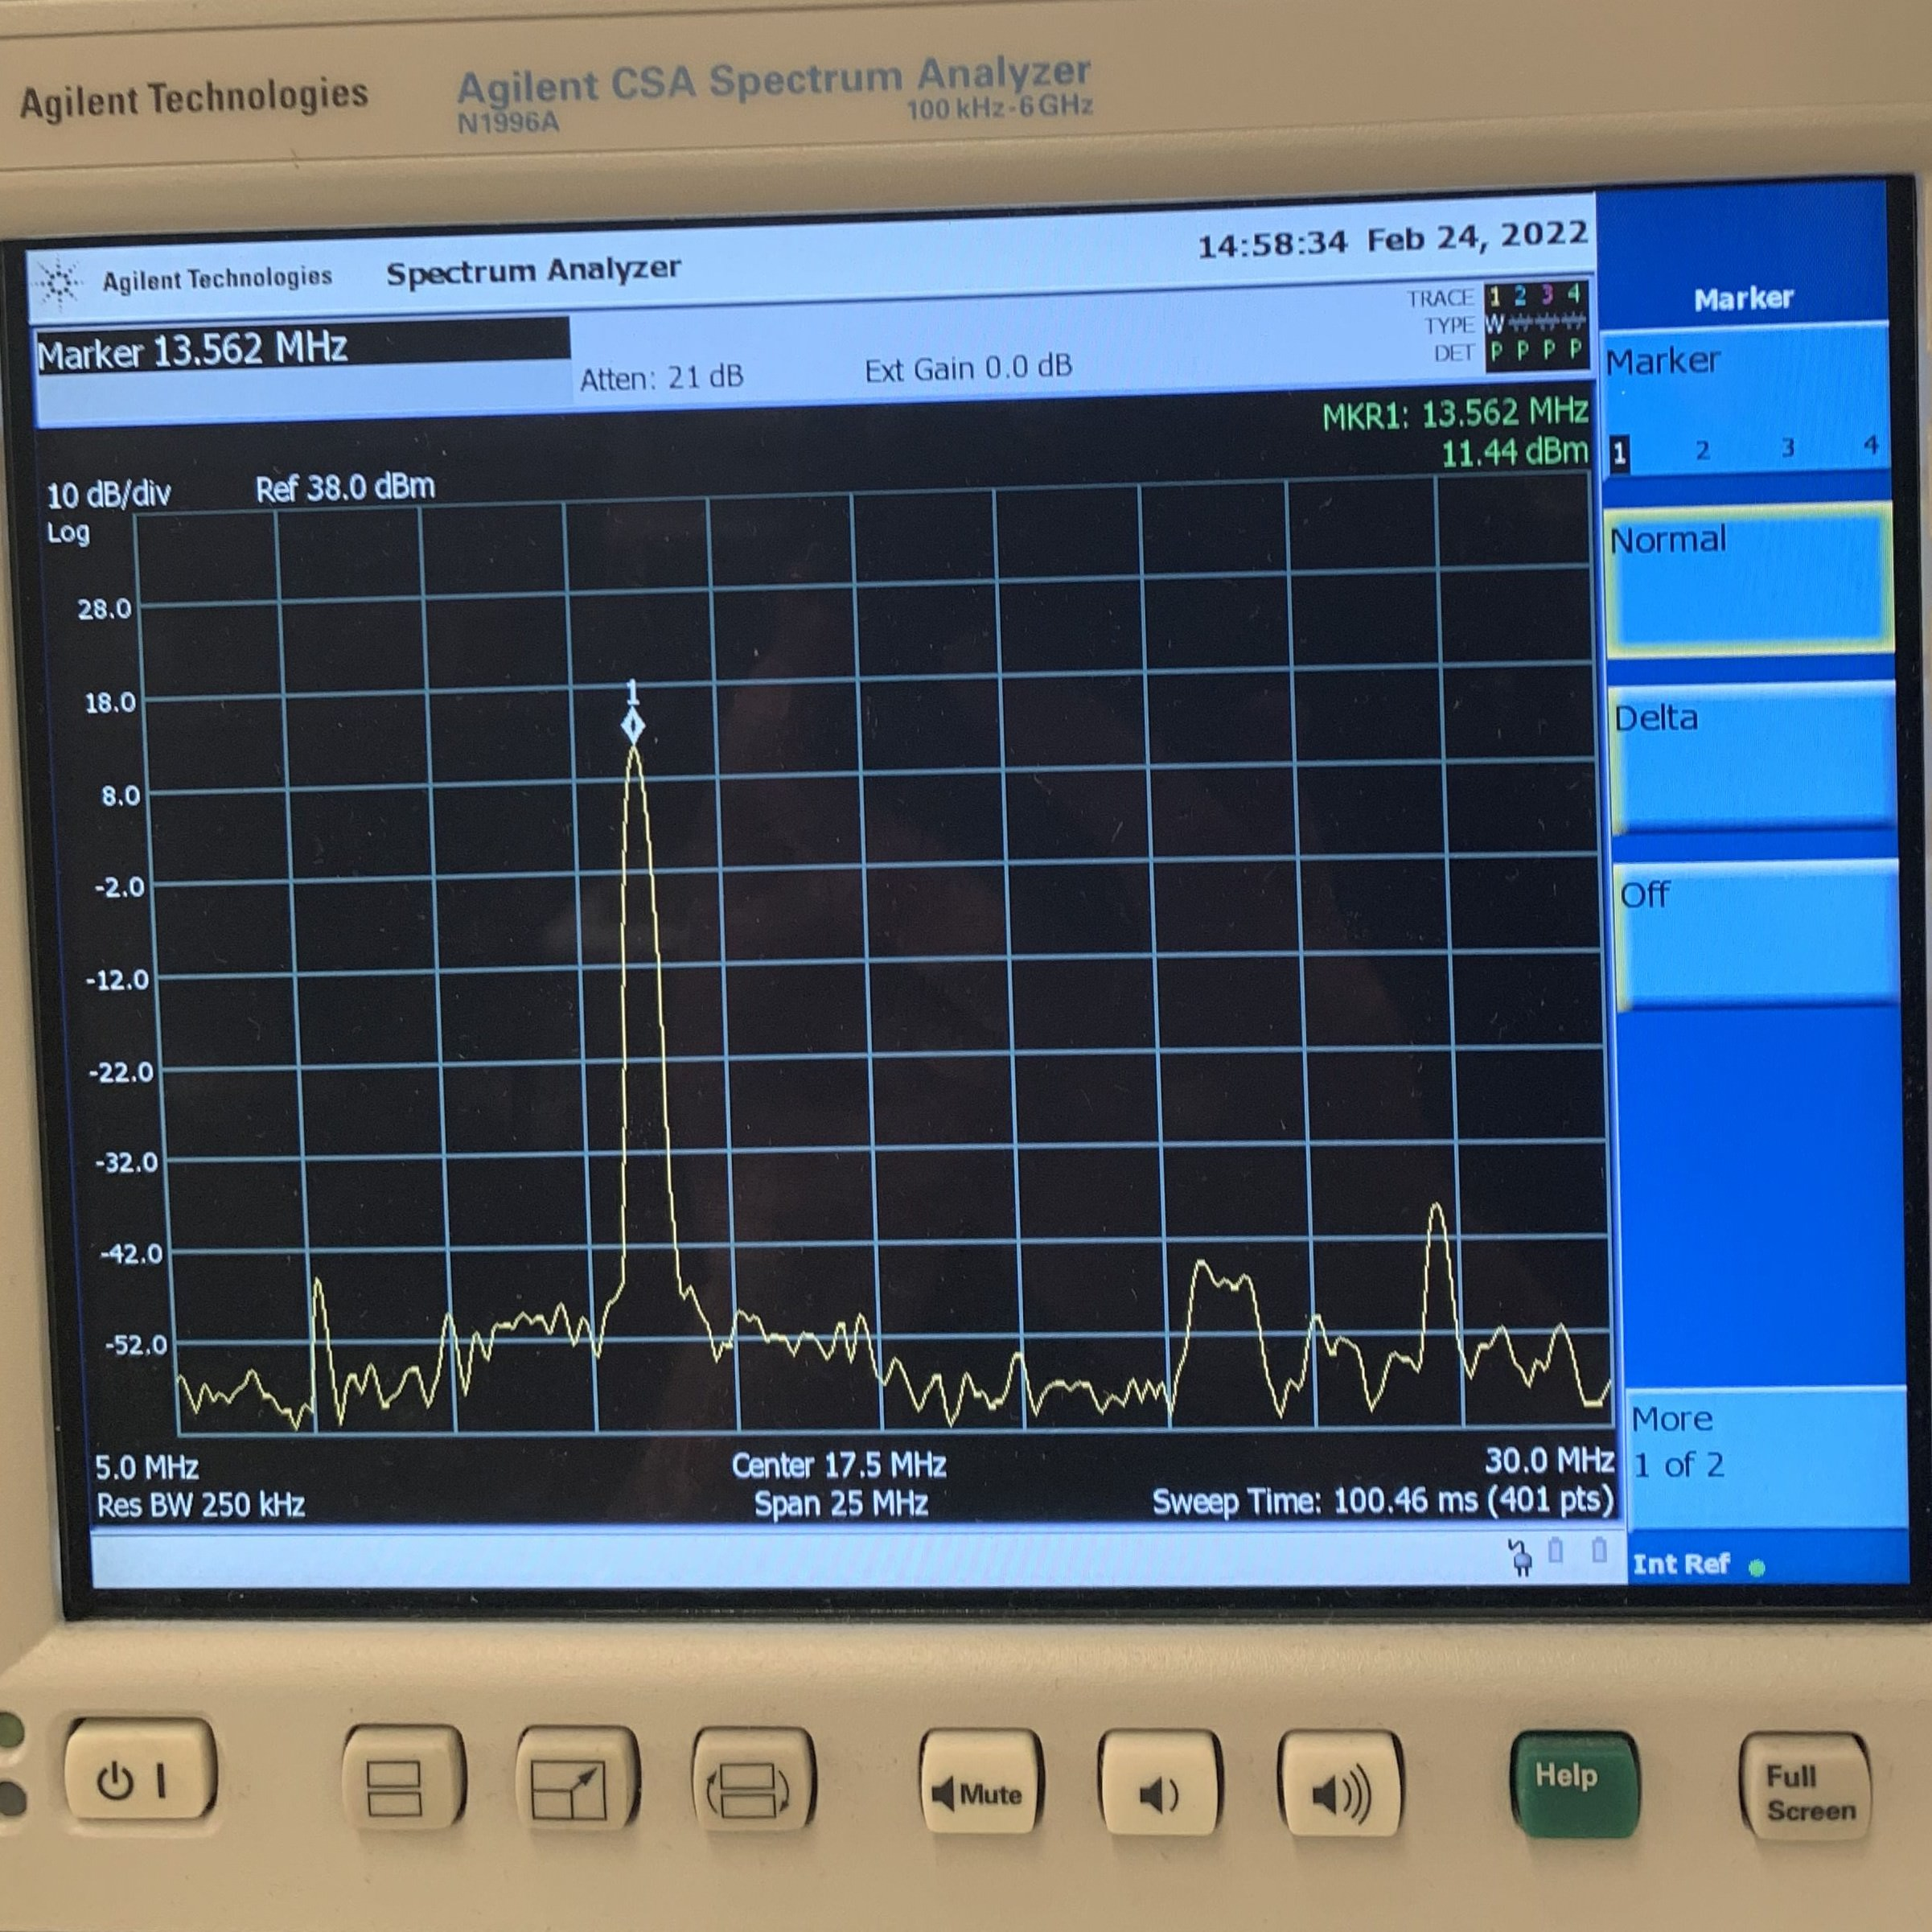
\includegraphics[width=2in]{14f}%
\label{fig_second_case}}
\hfil
\subfloat[]{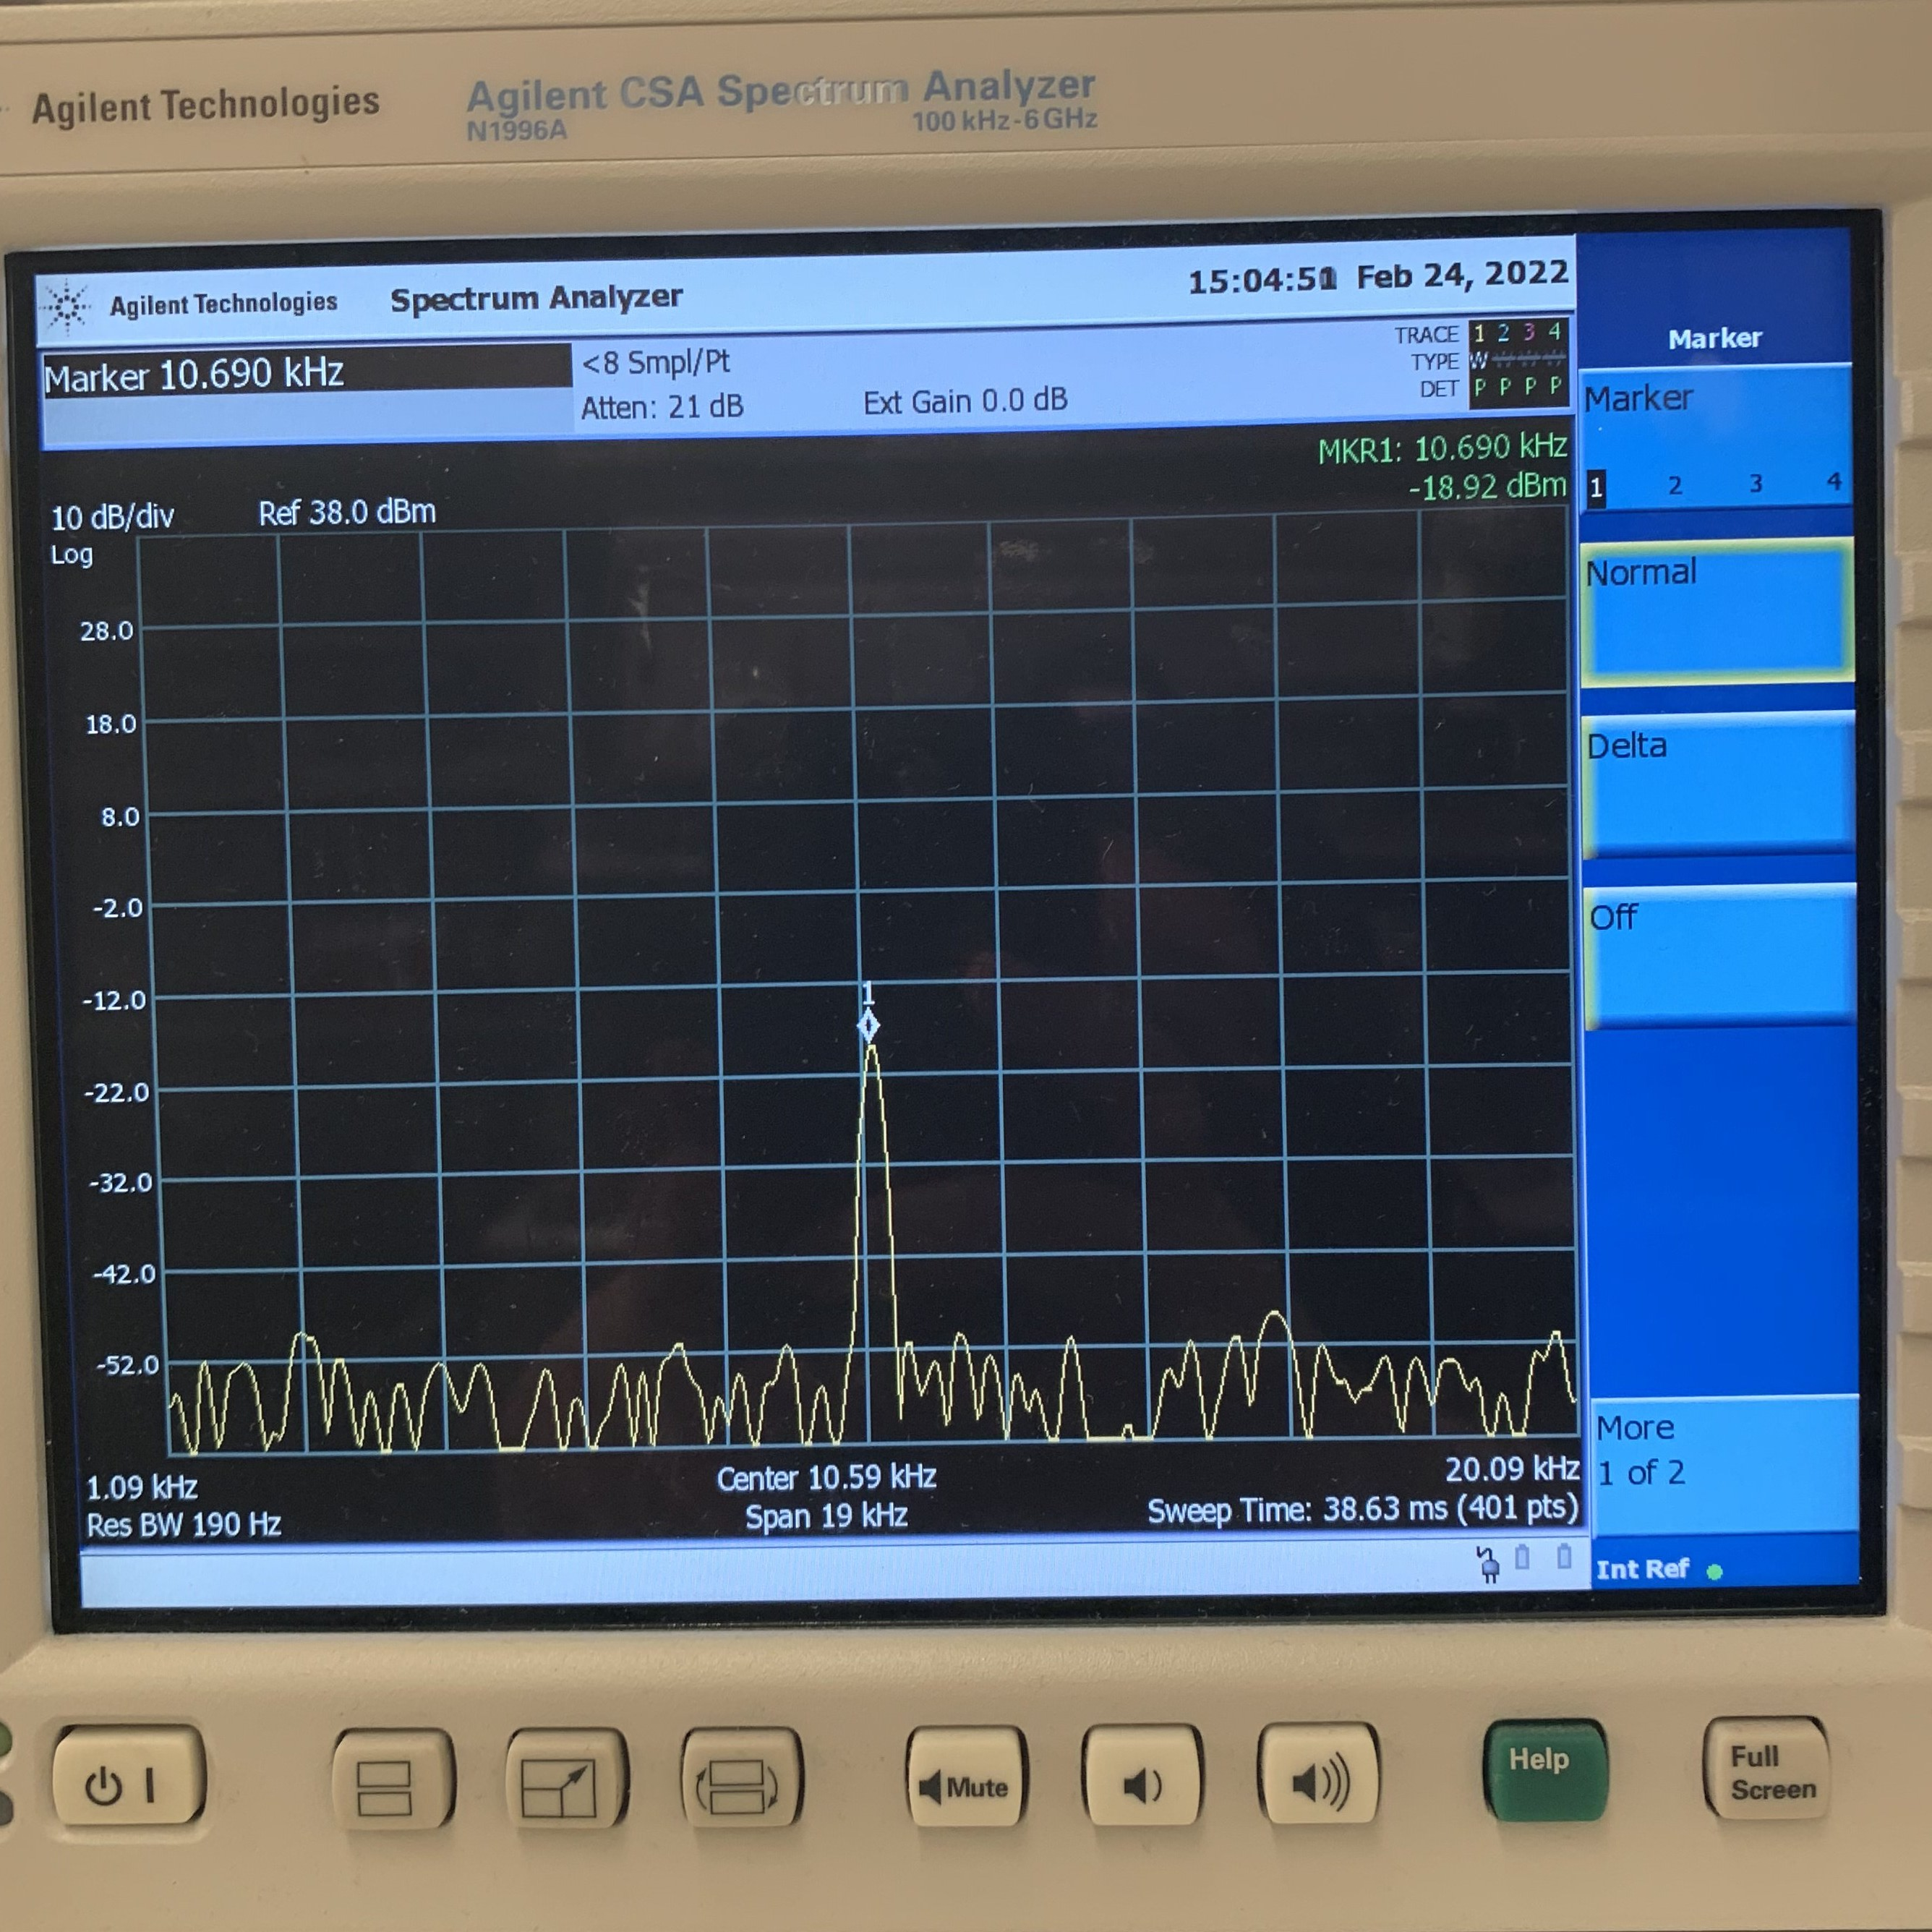
\includegraphics[width=2in]{11f}%
\label{fig_third_case}}
\caption{Frequency spectra, as seen with the spectrum analyzer. (a) $112.5 \,\text{MHz}$. (b) $13.55 \, \text{MHz}$. (c) $10.76 \, \text{kHz}$. Deviations from nominal peak frequencies can be seen in {\bf{Table 3}}.}
\label{fig_sim}
\end{figure*}

\section{Analysis}

After measuring the on the oscilliscope, we analyzed the waves using a spectrum analyzer. These Fourier-transformed spectra are available in Fig. 3.
The data comparing the measured peak frequencies to the nominal waveform frequencies are also available in {\bf{Table 3}}.

\section{Conclusion}

This lab explored wave form generation, visualization, and analysis using a simple and cheap setup. A clock generator and microcontroller were the essential components.

Despite this primitive setup, we found that the mesaured frequencies in all 6 tests we ran deviated from the nominal frequencies by less than 1\% each time. This is a remarkable result---and a testament to technological progress.

\section*{Acknowledgments}
Special thanks to my lab partners Devorah and Marc for all their help and support. They have lent several of their figures to match the data which I collected in my lab notebook. Thanks also to Yifan for inspiring me to dust off my \LaTeX skills, as well as helping with several of the Tikz schematics. Finally, thanks to Joanna and Steve for their endless patience in my quest to learn electronics.

%{\appendices
%\section*{Proof of the First Zonklar Equation}
%Appendix one text goes here.
% You can choose not to have a title for an appendix if you want by leaving the argument blank
%\section*{Proof of the Second Zonklar Equation}
%Appendix two text goes here.}


% \begin{thebibliography}{1}
% \bibliographystyle{IEEEtran}

% \bibitem{ref1}
% {\it{Mathematics Into Type}}. American Mathematical Society. [Online]. Available: https://www.ams.org/arc/styleguide/mit-2.pdf

% \end{thebibliography}

\end{document}


